\chapter{Fundamentação Teórica} \label{cpt:contexto}
Este capítulo descreve duas técnicas importantes que são relevantes para o desenvolvimento desta pesquisa. O \textit{framework} LODUS e a OpenAI API são os conteúdos abordados nas seções a seguir.

\section{\label{sec:back_lodus}LODUS}
LODUS é um \textit{framework} que permite simular ambientes urbanos virtuais em vários níveis de detalhes, tendo como objetivo principal prover informações para colaborar com os desafios de planejamento e manutenção de cidades~\cite{9239083}. O LODUS é um modelo multinível capaz de ser configurado de duas formas: i) reproduzindo cenários do mundo real ou ii) simulando dinâmicas urbanas antes de acontecerem na vida real. Em ambos os casos, é importante que o ambiente e a população possam ser coerentemente simulados.

O \textit{framework} permite a representação de um ambiente com diferentes níveis de abstração. Em cada nível, uma representação mais detalhada do ambiente pode ser definida, e a cada inclusão de um nível mais profundo, informações mais detalhadas podem ser computadas. Esses detalhes armazenam dados diversos, como distribuição populacional, sistema viário, geometria dos edifícios ou até mesmo configurações internas dos edifícios.

Dentro do LODUS, uma cidade pode ser definida por um Grafo de Região, esse grafo representa conexões entre regiões próximas. A Figura~\ref{fig:lodus}(a) abaixo demonstra a representação da cidade de Porto Alegre por um Grafo de Região, ao lado, a Figura~\ref{fig:lodus}(b) mostra a delimitação territorial da cidade no mundo real. Cada região do grafo está relacionada a um bairro dentro da cidade que possui seus pontos de interesse, por exemplo, casas, hospitais, postos de combustível, escolas e etc. Um ponto de interesse no ambiente tem suas características próprias e pode ser configurado no nível de detalhes desejado, por exemplo, pode se atribuir a um ponto de interesse a quantidade de pessoas nele e agrupá-las por idade, gênero, ocupação e etc. 

O \textit{framework} possibilita que dentro da simulação, pontos de interesse recebam populações de outros pontos de interesse com características especificas ou não, por exemplo, hospitais na região recebem populações que estão em casas, escolas, estádios de futebol e etc. Essas decisões de fluxo de população são parametrizáveis nas configurações.

\begin{figure}
    \centering
    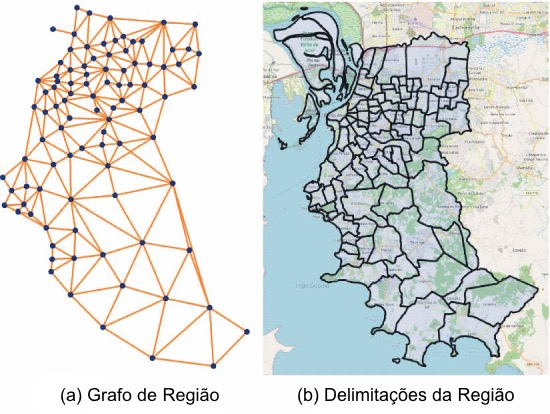
\includegraphics[width=12cm]{Capitulos/images/graph-region.jpeg}
    \caption{Grafo de Região do LODUS~\cite{9239083}.%GA: ref para a minha minha dissertação. Ajustar o crop da parte de baixo da imagem e esta com um pouco da legenda original.
    %GA: explicar as etapas na caption desta figura, mesmo que fique um pouco redundante com o texto (não copiar)
    %GA: As subfigures (que não são subfiguras no latex) estão com captions em inglês, tentar manter coerencia com o texto ou explicar o que é cada uma.
    }
    \label{fig:lodus}
\end{figure}

% \begin{figure}
%     \centering
%     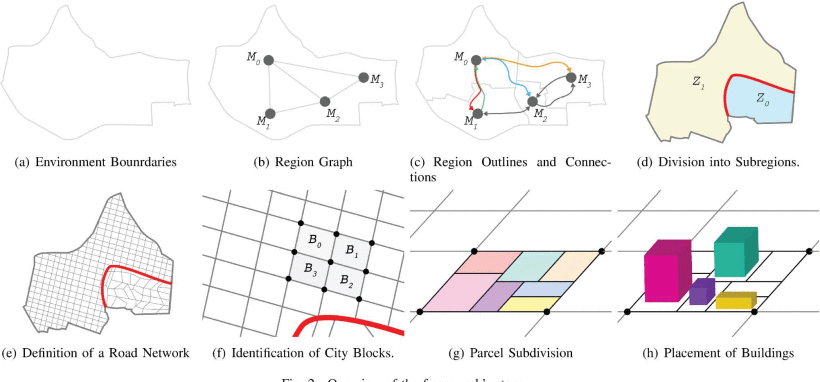
\includegraphics[width=\textwidth]{Capitulos/images/lodus-overview.png}
%     \caption{Visão geral dos estágios do framework.%GA: ref para a minha minha dissertação. Ajustar o crop da parte de baixo da imagem e esta com um pouco da legenda original.
%     %GA: explicar as etapas na caption desta figura, mesmo que fique um pouco redundante com o texto (não copiar)
%     %GA: As subfigures (que não são subfiguras no latex) estão com captions em inglês, tentar manter coerencia com o texto ou explicar o que é cada uma.
%     }
%     \label{fig:lodus}
% \end{figure}

% Na Figura~\ref{fig:lodus}(a), são ilustrados os Limites do Ambiente, representados em um plano 2D. Podemos definir o ambiente como um conjunto de Regiões, onde cada Região é um ponto 2D colocado dentro dos limites do ambiente. Uma Região pode representar diferentes áreas de acordo com o nível de abstração desejado, como: grupos de blocos da cidade dentro de um bairro; bairros dentro de uma única cidade; cidades dentro de uma área metropolitana; condados dentro de um estado; e estados dentro de um país.

% O Grafo de Região, conforme mostrado em Figura~\ref{fig:lodus}(b), pode ser especificado como um grafo não direcionado G=(P,E), onde P é um conjunto de nós (Regiões) e E contém um conjunto de arestas conectando os nós. Como um grafo planar pode ser aninhado dentro de um nó de outro grafo, é possível definir diferentes níveis de abstração para o Grafo de Região.

% Para permitir a criação de uma rede viária e a representação geométrica dos edifícios, cada região M também é representada por um Contorno (Figura~\ref{fig:lodus}(c)). O contorno de uma região é um polígono descrito por um conjunto de vértices que representam sua geometria.

% A seguir, uma conexão representa uma rota que permite o movimento de M\textsubscript{a} para M\textsubscript{b} por meio de uma lista ordenada de pontos 2D no espaço, onde cada ponto está dentro da geometria de O\textsubscript{a} $\cup$ O\textsubscript{b}. As conexões entre regiões são direcionais, mas podem ser usadas no sentido contrário se desejado pelo usuário e permitido pelas restrições do ambiente (ou seja, representação de rua de duas vias). Segmentos de uma conexão também podem ser compartilhados entre diferentes regiões para permitir movimento em rotas similares.

% Para representar o layout urbano em um nível mais baixo de abstração, é necessário estabelecer uma Rede Viária (Figura~\ref{fig:lodus}(e)) dentro de cada Região do ambiente. Uma Estrada (Q) é definida por uma lista de pontos 2D no espaço, onde cada par de pontos ([Q[i], Q[i+1]]) representa um segmento de estrada. Um conjunto de pontos em uma estrada pode ser compartilhado com um Contorno, permitindo que a estrada represente os limites de uma Região. Para preservar as propriedades de um grafo planar herdadas pelo Grafo de Região, os segmentos de estrada não podem se cruzar. Em casos de interseções, um novo ponto é colocado no ambiente e a lista em cada estrada é ajustada para compreender o novo segmento. Apesar de compartilharem a mesma estrutura, o framework distingue as estradas em "primárias" (ou seja, estradas arteriais, avenidas principais ou rodovias) e "secundárias" (ou seja, ruas locais), devido aos seus propósitos em cada etapa.

% As estradas primárias atravessam grandes partes do contorno de uma Região e são responsáveis por dividir o contorno em Subregiões (Figura\ref{fig:lodus}(d)), representando uma segmentação de um Contorno. As estradas secundárias fornecem acesso local para diferentes áreas dentro de uma Subregião e podem ter um comprimento menor. Os pontos extremos de uma estrada primária devem pertencer ao contorno da Região ou a outra estrada primária. Essa restrição é aplicada para manter as propriedades do grafo planar. Um conjunto de parâmetros é definido para descrever as estradas em maior detalhe e permitir a integração com outras aplicações, por exemplo, simulação de tráfego.

% Após a formação da rede de estradas secundárias, é possível obter um conjunto de quadras (Figura\ref{fig:lodus}(f)) dentro de cada Subregião. Uma quadra também é representada por um conjunto de pontos 2D formando um polígono. Cada ponto em uma quadra pertence a um segmento de estrada secundária ou ao contorno da Subregião. As quadras compreendem um conjunto de lotes (Figura\ref{fig:lodus}(g)), que são usados como base para a geração de edifícios e casas (Figura\ref{fig:lodus}(h)). As quadras dentro da mesma Subregião podem compartilhar um conjunto padrão de propriedades para dar a elas uma aparência semelhante. Como uma quadra pode conter vários lotes, um algoritmo de subdivisão é aplicado às quadras desejadas com uma área grande o suficiente.



%GA: no caso deste trabalho, acho que a movimentação entre regiões e bairros é mais relevantes de comentar, pq tu não chega a utilizar as ruas em si ou uma API de rotas
Nesta pesquisa, o LODUS é utilizado como ferramenta central no desenvolvimento do modelo de simulação. Um ambiente simulando os bairros, ruas e estradas da cidade de Porto Alegre é empregado, e um \textit{plugin} customizado é adicionado para possibilitar o contexto de fluxo de ocupação hospitalar dentro da simulação.

\section{\label{sec:chat}OpenAI API}
A API da OpenAI oferece acesso a poderosas ferramentas de inteligência artificial desenvolvidas pela OpenAI. Ela permite que os desenvolvedores integrem facilmente modelos de linguagem avançados, como o GPT-3 (\textit{Generative Pre-trained Transformer})~\cite{brown2020language}, em suas próprias aplicações. %GA: tem alguma ref para o GPT-3? acho que deve ter algum paper publicado deles (GV: corrigido)
Atualmente, a API fornece uma interface ``\textit{text in, text out}'' de propósito geral, possibilitando a integração da API em produtos existentes, novas implementações ou ajudando a OpenAI a explorar os limites dessa tecnologia~\cite{OPENAI}.

Dado qualquer \textit{prompt} de texto, a API retornará um texto de resposta, tentando corresponder ao padrão fornecido. A API pode ser programada a partir de alguns exemplos nos quais o usuário gostaria que o resultado fosse semelhante, e a qualidade dos resultados geralmente varia dependendo da complexidade da tarefa. Além disso, a API permite aprimorar o desempenho em tarefas específicas com o treinamento de conjuntos de dados de exemplos fornecidos ou por meio de \textit{feedback} humano de usuários ou rotuladores. Ela pode ser aplicada em diversos contextos para enriquecer a interação humano-computador. A seguir está listada uma visão simplificada do funcionamento da API.

\begin{itemize}
    \item Requisição e Autenticação: Um usuário envia uma solicitação para a API da OpenAI, geralmente contendo um \textit{prompt} de entrada, que é o texto inicial para o qual deseja uma resposta. A autenticação é realizada usando credenciais de API, garantindo que apenas usuários autorizados tenham acesso.

    \item Processamento: A API recebe a solicitação e a processa internamente. Isso envolve analisar o \textit{prompt} de entrada, entender o contexto e determinar qual modelo de linguagem e quais parâmetros usar para gerar uma resposta adequada.

    \item Modelo de Linguagem: A API utiliza modelos de linguagem avançados, como o GPT, para gerar respostas. Esses modelos são treinados em grandes conjuntos de dados para entender a estrutura da linguagem natural e gerar texto coerente e relevante.

    \item Geração de Resposta: Com base no \textit{prompt} de entrada, o modelo de linguagem gera uma resposta correspondente. Isso envolve a geração de texto novo, seguindo o contexto fornecido pelo \textit{prompt}, bem como qualquer informação adicional, como configurações específicas do modelo.

    \item Retorno da Resposta: A resposta gerada pelo modelo é então enviada de volta ao usuário como a saída da API. Isso geralmente acontece em tempo real, dependendo da complexidade da solicitação e da carga de trabalho do servidor.

\end{itemize}

Em resumo, a API da OpenAI utiliza modelos de linguagem avançados para compreender e gerar texto em resposta às solicitações dos usuários, oferecendo uma interface simples para a integração de inteligência artificial em uma variedade de aplicativos e cenários. A Figura~\ref{fig:openai-flow} apresenta, de maneira geral, um exemplo do fluxo de comunicação com a API.

\begin{figure}
    \centering
    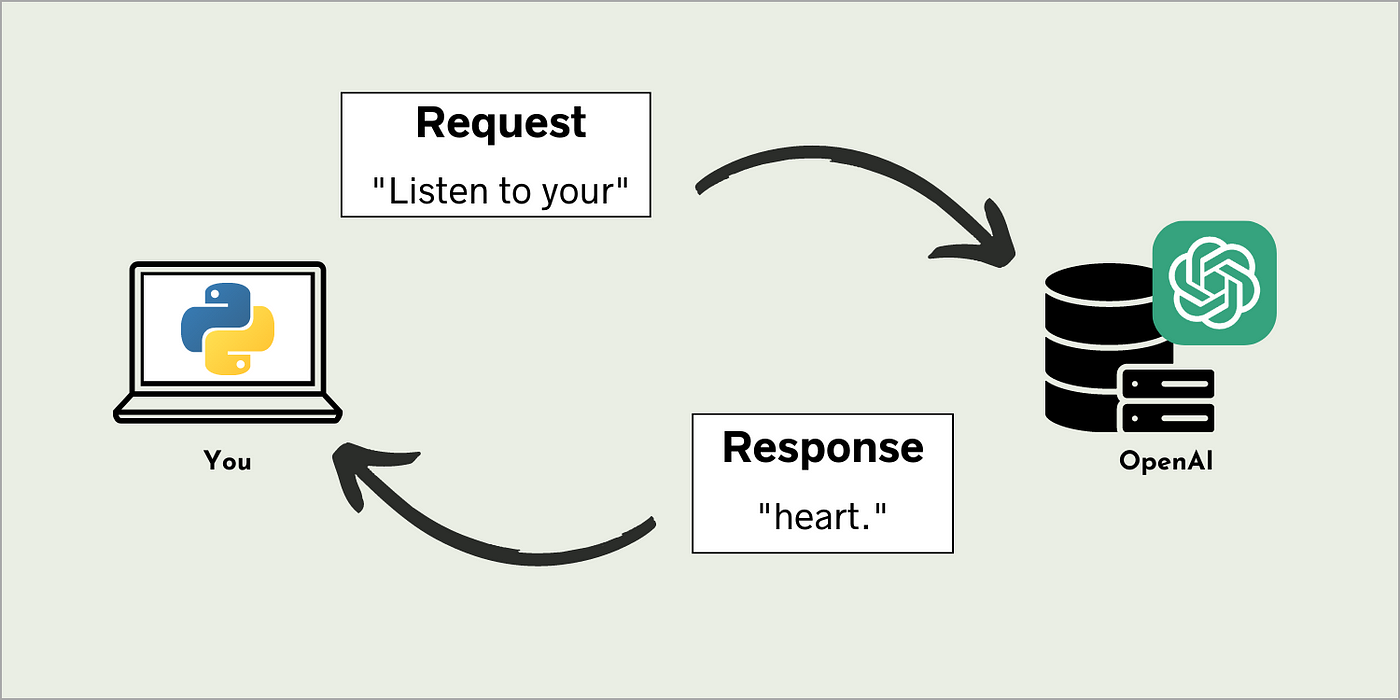
\includegraphics[width=0.75\textwidth]{Capitulos/images/openai-api.png}
    \caption{Fluxo de comunicação da API~\cite{OPENAIIMAGE}.}
    \label{fig:openai-flow}
\end{figure}

No desenvolvimento desta pesquisa, a API é utilizada para a geração de textos de internação hospitalar para uma determinada especialidade de internação selecionada pelo usuário na interface, dependendo dos parâmetros de configuração utilizados na simulação.